% Copyright (C) 2020 by Landmark Acoustics LLC

\documentclass[preprint]{JASA}

\begin{document}
%% the square bracket argument will send term to running head in
%% preprint, or running foot in reprint style.

\title[Efficiently Generating AR Power Law Noise]
{Quantifying the Efficiency of Autoregressive Generators of Power Law Noise}

\author{Benjamin N. Taft}

\affiliation{Landmark Acoustics LLC, Racine, WI 53405, USA}

\email{ben.taft@landmarkacoustics.com}

\date{\today} 

\begin{abstract}
  Power law noise, in which the energy at each frequency is related to the   power of that frequency, is ubiquitous in nature.
  Signal detection algorithms, therefore, should often be tested in the context   of noise with different ``colors'', or exponents, of power law noise (PLN).
  These noise colors range from ``red,'' when the frequency exponent is -2,   through ``white,'' when the exponent is 0, to ``blue,'' which has an exponent  of 2.
  There are many algorithms for generating realistic PLN.
  Generators that use autoregressive (AR) functions are particularly useful because they are reasonably intuitive and can be parameterized to generate the full range of PLN ``colors.''
  In principle, the degree, or number of terms, in the AR generator for any color of PLN may be infinite.
  In practice, there are theoretical caps on the degree for some exponents, and diminishing returns for increasing the degree for others.
  This article demonstrates quantitative decision rules for choosing the degree for a discrete AR generator of PLN based on the size of the noise vector
  being generated and the tolerence its user has for slight deviations between the realized power law and the desired exponent.
\end{abstract}

\maketitle

\section{Introduction}

Power law noise is a time series where the energy at different frequencies is a function of the frequency raised to a power.
True red noise has a power of -2, true white noise has a power of 0, and true violet noise has a power of 2.
Pink noise has a power between -2 and 0, exclusive.
Blue noise has a power between 0 and 2, exclusive.
There are many ways to generate power law noise.
A particularly useful one uses an autoregressive model where the weights given to previous values of the time series are a function of the power and a
decreasing function of the time lag to the term.
Some powers have a fixed number of non-zero terms.
White noise, for example, has no non-zero terms, and true red noise has only one.
All other powers have a potentially infinite number of terms.
The actual number of terms in an autoregressive model is its degree.
Obviously, there are diminishing returns to increasing the degree of a model.
This project is aimed at finding a rule for choosing how big a model's degree should be.
The rule will be quantified according to the difference that one is willing to tolerate between the observed spectral slope and the expected slope of the spectrum of the time series.

There are three crucial parameters that I want to examine:
\begin{description}
\item[$\alpha$] The power of the power law.
  When the spectral energy at a
  frequency $f$ is  $S(f)$ then $S(f) \propto f^{\alpha}$.
\item[$N$] The number of samples in the time series
\item[$K$] The degree of the autoregressive model
\end{description}

It is useful to be able to generate power law noise in a controlled way.
Power law noise shows a roughly linear relationship between the logarithms of frequency and amplitude.
That is to say, the distribution of energies ($P$) across frequencies ($f$) is governed by a parameter ($\alpha$) such that $P \propto f^{\alpha}, \alpha \in
\mathbb{R}$.
By analogy with mixtures of light energy, the slope of the relationship between frequency and amplitude in a sample of power law noise is often referred to by color.
Red noise has a slope, or $\alpha$, near -2, pink noise's slope is -1, white's is 0, blue's is +1, and violet's is 2.
Natural sounds and speech often occur in an environment of noise with an energy distribution somewhere between pink and white.
That is, there is more energy in the lower frequencies of these environments' background noise.
Room acoustics have pink power law noise because of reverberation \citep{summers:2013}.
Aquatic acoustic environments are filled with pink noise from both shipping \citep{helbleetal:2012} and natural processes.
Algorithms for detecting features of speech or animal sounds should therefore be examined in the presence of power law noise \citep{skowronski:fenton:2008}.

Feature extractors should have well-understood responses to the kinds of power law noise that they are likely to encounter in the wild \citep{beckham:austin:1975}.
One way of doing this would be to mix test sounds with natural recordings of power law noise.
This has the disadvantage of depending on the availability and quality of noise recordings.
Any such recordings also necessarily conflate the frequency content of the background noise with the frequency response of the recording system.
It can also be difficult to predict how well an algorithm that has been trained to work in specific recordings of background noise will generalize to different real-world situations.
Using artificially generated noise can solve these problems because the user can dictate an algorithm's parameters to match the full range of cases expected in the real world.

Published algorithms that generate discrete-time power law noise seem to fall into two approaches.
One approach, is essentially a finite impulse response (FIR) filter \citep{kasdin_walter:1992}.
It uses two discrete Fourier Transforms to manipulate a batch of samples in the frequency domain \citep{zhivorimov:2018}.
That is,
\begin{equation}
  \mathbf{x} = \mathcal{F}^{-1}\left\{\mathbf{h}\,\mathcal{F}\{\mathbf{n}\}\right\},
\end{equation}
where $\mathbf{x}$ is a vector of power law noise, $\mathcal{F}\{\cdot\}$ is the discrete Fourier transform, $\mathbf{h}$ is a vector that describes the desired distribution of energy in the output noise, and $\mathbf{n}$ is a vector of random values from the standard normal distribution.
An FIR approach therefore requires approximately $O(N \log N)$ calculations to generate $N$ samples of power law noise.
This makes the FIR approach extremely efficient \citep{zhivorimov:2018}.
However, it produces its noise in batches of fixed length.
If you do not know how many samples you need beforehand, or if $N$ is extremely large, the FIR approach may not be practical.
Another approach, uses autoregression (AR) models to generate new noise samples as a function of preceding samples \citep{pachet:etal:2015}.
That is,
\begin{equation}
  x_i = n_i + \sum_{k=1}^Ka_kx_{i-k},
\end{equation}
where $\mathbf{a}$ is a vector of coefficients from an AR generator of degree $K$.
Thus an AR generator of degree $K$ requires approximately $O(NK)$ calculations to generate $N$ samples of power law noise.
Consequently, the AR approach takes more computations than the FIR approach when $K>\log N$.
However, the AR may still be better-suited to online applications because it generates power law noise one sample at a time, rather than all at once.

One AR generator of discrete power law noise is described by \citet{kasdin_walter:1992}, and calculates each term as a ratio of rising factorials of $\frac{\alpha}{2}$ and $k$:
\begin{equation}
  a_k = \frac{(\frac{\alpha}{2})_k}{k!} = \frac{\prod_{i=0}^{k-1}{\frac{\alpha}{2}+i}}{k!} = \frac{\Gamma(\frac{\alpha}{2}+k)}{\Gamma(\frac{\alpha}{2})k!}=\frac{1}{k\mathrm{B}(\frac{\alpha}{2},k)}\text{.}
\end{equation}
\citet{kasdin1995discrete} points out a convenient recursive way to generate the generator's terms:
\begin{equation}
  a_k = \prod_{i=1}^{k}\frac{\frac{\alpha}{2}+i-1}{i}\text{.}
\end{equation}

There should be diminishing returns to adding more terms to an AR generator, but the rate at which the returns decrease should depend on the value of $\alpha$.
The minimum efficient degree of an AR generator depends on the exponent of the power law noise being generated because different exponents correspond to generators that make use of different amounts of past information.
Brownian noise, when $\alpha = -2$, only requires a degree of one because $a_1 = -1$, and $a_k$ is zero otherwise.
This makes sense because Brownian noise is made by adding a new sample of white noise to a running total of previous samples.
Similarly, white noise, when $\alpha = 0$, is a zero-degree generator because $a_1 = 0$.
This also makes sense because white noise doesn't use any previous information, just a new sample of Gaussian noise.
However, for violet noise, when $\alpha = 2$, there is no obvious cutoff because $a_k = 1$ for all $k$.
This might correspond to noise from an infinite feedback loop
These observations suggest that the minimum effective degrees of the generator should be a function, $\hat{K}(\alpha)$, defined on $-2 \le \alpha < 2$.
Furthermore, the function should be continuous, pass through $(-2, 1)$ and $(0, 0)$, have a local maximum somewhere in $-2 < \alpha < 0$, a local minimum at $\alpha = 0$, and then increase towards a vertical asymptote at $\alpha=2$.

Kasdin demonstrated a recursive formula for creating a discrete AR generator of power law noise \citep{kasdin_walter:1992}.
The number of terms in the generator, $K$, is its degree.
The $n$th term of a discrete autoregressive generator for noise with a power law of $\alpha$ is
\begin{equation}
  \label{iterative_term}
  h\left(\alpha, n\right) =
  \frac{{\left(\frac{\alpha}{2}\right)}_n}{n!} =
  \frac{\prod_{k=0}^{n-1}{(\frac{\alpha}{2}-k)}}{n!} =
  \frac{\Gamma\left(\frac{\alpha}{2}+n\right)}{\Gamma\left(\frac{\alpha}{2}\right)n\Gamma\left(n\right)} =
  \frac{1}{n\mathrm{B}\left(\frac{\alpha}{2},n\right)}.
\end{equation}
There are diminishing returns to increasing the degree of the generator, and this paper looks for a way to compute the smallest appropriate degree for any particular application of the generator.
To quantify `smallest appropriate degree,' I will compare the expected log-log slope of the noise's spectrum, $\alpha$, to the actual slope, $m$.
The closer the match between $\alpha$ and $m$, the better the generator, so the quantity we are trying to minimize is $\left|\alpha - m\right|$, or, equivalently, $\sqrt{\left(\alpha - m\right)^2}$.

We control four things when we generate power law noise: the exponent of the power law, $\alpha$, the degree of the generator, $K$, the length of the time series output, $N$, and the amount of error that we are willing to tolerate, $\epsilon$.
For the applications that I am considering, $\alpha$, $N$, and $\epsilon$ will be driven by the question under investigation.
By minimizing $K$ within the context of those constraints, we can minimize our use of time and/or computational resources.

I expect the error for a particular parameterization of the generator, $E_{\alpha}(N, K)$ to asymptotically decrease as $N$ and $K$ increase.
A useful equation for describing that relationship is
\begin{equation}
  \label{error_fit}
  E(\alpha) = B_0(\alpha)
  + \frac{B_1(\alpha)}{\sqrt{N}}
  + \frac{B_2(\alpha)\sqrt{N}}{K}
\end{equation}

The key insight is \textbf{Degree Ratio}, which is $\frac{K}{\sqrt{N}}$.
This has really nice properties.
First, its limit is straightforward:
\begin{equation}
  \lim_{K \to \infty}{E(\alpha)} = B_0(\alpha) + \frac{B_1(\alpha)}{\sqrt{N}}
\end{equation}

which means we can use epsilon-delta to look for a degree that is arbitrarily
close to this limit:
\begin{equation}
  \lim_{\delta \to 0}{\frac{B_2(\alpha)\sqrt{N}}{K+\delta}} < \epsilon
\end{equation}

which simplifies to:
\begin{align}
  B_2(\alpha)\sqrt{N} & < \epsilon({K + \delta}) \\
  B_2(\alpha)\sqrt{N} & < \epsilon K + \epsilon\delta \\
  B_2(\alpha)\sqrt{N} & < \epsilon K \\
  \epsilon K & > B_2(\alpha)\sqrt{N} \\
  K &> \frac{B_2(\alpha)\sqrt{N}}{\epsilon}
\end{align}

\section{Methods}

\subsection{Simulations}

I used a custom Python module to simulate multiple realizations of the power law generator in which I varied the exponent of the power law ($\alpha$), the length of the output series ($N$), and the degree of the autoregression generator ($K$).
The values of $\alpha$ ranged from -2 to 2, with an interval of 0.02.
As described above, I was testing the hypothesis that the exponent ($\alpha$) and  degree ratio ($K/\sqrt{N}$) of an AR generator are the key quantities for determining its optimal degree.
For that reason, the output size and degree of each simulation were not independent.
I wanted to test degree ratios between 1/20 and 20.
This meant that the smallest $N$ was near 400, the smallest number for which a degree ratio of 1/20 is at least one.
The largest $N$ was near 5000, which I chose arbitrarily as the largest output size that I would deal with.
The actual values of $N$ that I used were the integers in the range [400, 5000] that were composite multiples of only 2 and 3.
The actual output sizes consisted of twenty-seven values between 432 ($2^43^3$) and 4608 ($2^93^2$).
The degrees thus ranged from 1 to 416 when $N=432$ and from 1 to 1358 when $N=4608$. 
I used twenty iterations for each combination of exponent, output size, and degree for a total of 14,853,900 simulations.

In each simulation, I computed the frequency spectrum of each series, and then found the slope (called $m$), of the best-fit line through its log-log representation.
I calculated each simluation's error as the absolute value of the difference between the its observed power law and its $\alpha$ value.
\begin{equation}
  \label{error_definition}
  E = \left|m - \alpha\right|.
\end{equation}
The final data set contained the values Exponent ($\alpha$), Size ($N$), Degree ($K$), Slope ($m$), and Slope Error ($E$) for each simulation.

\subsection{Model Fitting}

The final goal of this study is to find a formula for calculating an efficient degree for an autoregressive generator of power law noise.
The inputs to this formula are the models exponent ($\alpha$), its size ($N$), and the amount of error that the user is willing to tolerate ($\epsilon$).

Using the simulations described above, the first step toward finding this formula is to find an expression that predicts the absolute difference between the desired power law ($\alpha$) and the observed power law ($m$), or the generator's slope error ($E$).
I fit a generalized linear model of $E$ for each value of $\alpha$ in the simulations, using the same formula each time:
\begin{equation}
  \label{glm_of_error}
  E \sim B_0 + B_1\frac{1}{N} + B_2\frac{\sqrt{N}}{K} + e
\end{equation}
The models each contained four terms: an intercept term, an inverse size term, an inverse degree ratio term, and an error term.
Using the \texttt{glm} method in \texttt{R}, I treated the error term as Gamma distributed, with  a log linking function \citep{rcoreteam:2020}.
Based on the algebra above, the key to estimating the most efficient degree of a generator is the inverse degree ratio term.

The second step toward finding a formula for an efficient degree is to create a model that estimates the inversed degree ratio term as a function of a generators exponent.
There previous step yielded 201 estimates for $B_2(\alpha)$, just one for each exponent value.
I used \texttt{R}'s \texttt{lm} function to fit polynomial regressions of the form
\begin{equation}
  \label{coefficient_model}
  B_2(\alpha) \sim \sum_{i=0}^{20}{\beta_i \alpha^i}
\end{equation}
I used \texttt{R}'s \texttt{step} methods to find the most parsimonious combination of coefficents.
I fit two separate polynomials, one for pink noise ($\alpha <= 0$), and one for blue noise ($\alpha >= 0$).

\section{Results}
\section*{Discussion}

A time series is called power law noise when its future values have some randomness to them but also depend on past values from the time series.
A signal is power law noise with exponent $\alpha$ when the energy of its frequency spectrum, $S(f)$, is proportional to $f^{\alpha}$ at each frequency $f$.
On a log-log plot, a best-fit line through such a spectrum has a slope of $\alpha$.

The excellent thing about this is that it comes back to degree ratio: 
\begin{equation}
  \frac{K}{\sqrt{N}} = \frac{B_2(\alpha)}{\epsilon}
\end{equation}

I can estimate the coefficients of equation \ref{error_fit}, $\mathbf{b}_{\alpha}$, with an empirical approach.

\begin{figure}[ht]
  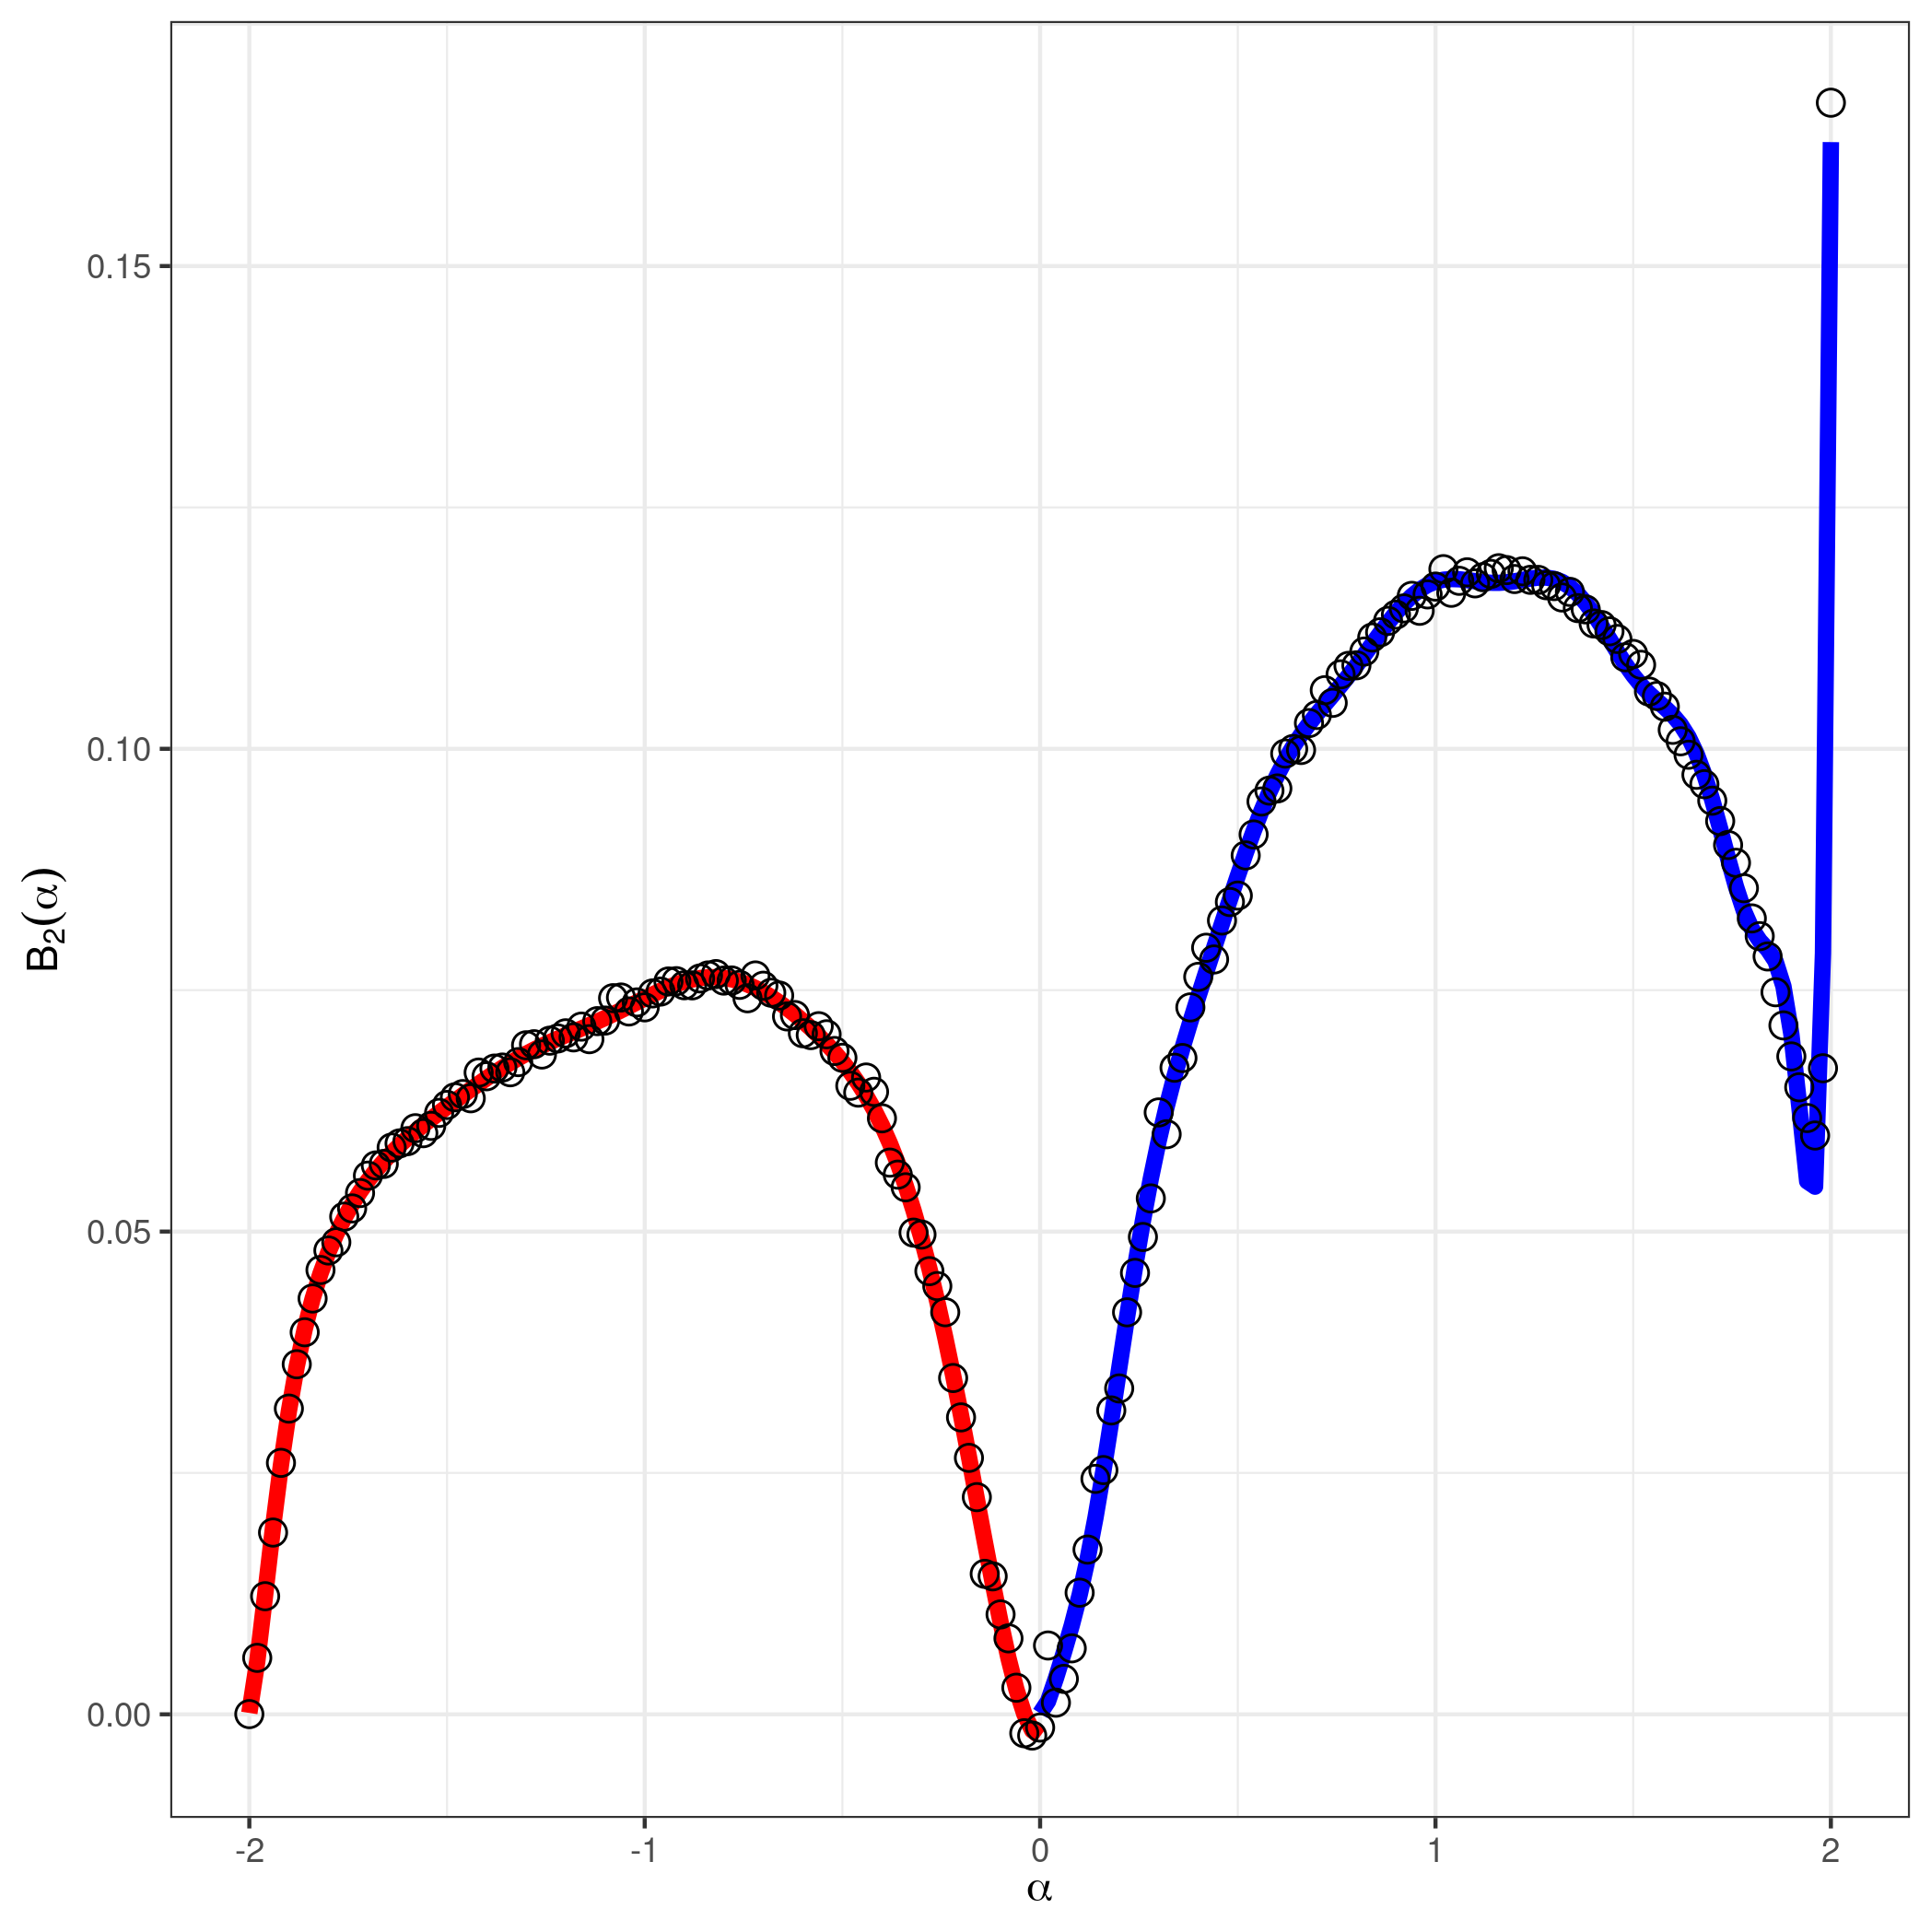
\includegraphics[width=\reprintcolumnwidth]{Figure3}
  \caption{\label{fig:DegreeRatioCoefs}{
      The coefficients of the inverse Degree Ratio ($\sqrt{N}/K$) terms from
      the models that relate the Slope Error of simulated PLN to the size and
      degree of the generator.
    }}
\end{figure}

\begin{table}[ht]
  \caption{\label{tab:pink_model_coefficients}
    The coefficients to the polynomial fit between a ``pink'' noise generator's
    exponent ($\alpha <= 0$) and the Degree Ratio term in the model of that
    generator's Slope Error.
  }
  \begin{ruledtabular}
    \begin{tabular}{cc}
      Exponent & Coefficient\\
      \hline
      Intercept & -0.00227314914613336\\
      2 & 1.63031943883604\\
      3 & 4.98482144802658\\
      4 & 4.97536531055866\\
      7 & 4.21645358084128\\
      10 & 20.0002829702428\\
      11 & 36.311281476006\\
      12 & 27.0101728835473\\
      13 & 8.52755459477657\\
      15 & -0.531541800533245\\
      17 & 0.031440622365535\\
      20 & 0.000291974320416611\\
    \end{tabular}
  \end{ruledtabular}
\end{table}

\begin{table}[ht]
  \caption{\label{tab:blue_model_coefficients}
    The coefficients to the polynomial fit between a ``blue noise generator's
    exponent ($\alpha > 0$) and the Degree Ratio term in the model of that
    generator's Slope Error.
  }
  \begin{ruledtabular}
    \begin{tabular}{cc}
      Exponent & Coefficient\\
      \hline
      Intercept & 9.4196455046796e-05\\
      2 & 4.41910305885241\\
      3 & -79.5386727156783\\
      4 & 818.799633843592\\
      5 & -4841.87374846092\\
      6 & 17902.4307608028\\
      7 & -44065.3564402454\\
      8 & 74941.2141298672\\
      9 & -89603.5421646984\\
      10 & 75260.5594029616\\
      11 & -43364.831286192\\
      12 & 16030.1475015981\\
      13 & -3098.55090428394\\
      15 & 100.084618948057\\
      17 & -3.86836146896404\\
      20 & 0.0236495550796521\\
    \end{tabular}
  \end{ruledtabular}
\end{table}

\begin{acknowledgments}
  This research was supported by Landmark Acoustics LLC.
\end{acknowledgments}

% =======================================================

\bibliography{power_law_noise}

% =======================================================

\end{document}

